\documentclass[11pt,a4paper]{article}
\usepackage[T1]{fontenc}
\usepackage[utf8]{inputenc}
\usepackage{lmodern,microtype,graphicx,booktabs,tabularx,array,amsmath,amssymb}
\usepackage[margin=22mm]{geometry}
\usepackage[colorlinks=true,linkcolor=black,citecolor=black,urlcolor=blue]{hyperref}
\usepackage[numbers,sort&compress]{natbib}
\usepackage{caption,float}
\usepackage[section]{placeins}
\captionsetup{font=small,labelfont=bf}
\renewcommand{\topfraction}{0.95}
\renewcommand{\bottomfraction}{0.9}
\renewcommand{\textfraction}{0.05}
\renewcommand{\floatpagefraction}{0.8}
\widowpenalty=10000
\clubpenalty=10000
\setlength{\parskip}{4pt}
\setlength{\parindent}{12pt}
\setlength{\emergencystretch}{1.5em}
\newcommand{\co}{CO\textsubscript{2}}
\newcommand{\rr}{CO\textsubscript{2}RR}
\newcommand{\ca}{Cu--Au}
\title{An agentic framework for X-ray absorption spectroscopy of catalytic interfaces}
\author{Haili Jia and Maria K. Y. Chan\thanks{Corresponding author. E-mail: \href{mailto:mchan@anl.gov}{mchan@anl.gov}.}\\[0.6em]
\small Center for Nanoscale Materials, Argonne National Laboratory,\\
\small 9700 South Cass Avenue, Lemont, Illinois 60439, United States}
\hypersetup{pdftitle={An agentic framework for X-ray absorption spectroscopy of catalytic interfaces},pdfauthor={Haili Jia and Maria K. Y. Chan}}
\date{}
\begin{document}
\maketitle
\begin{abstract}
Designing selective catalysts requires understanding how local atomic environments stabilize intermediates and redirect competing reaction pathways. X-ray absorption spectroscopy (XAS), including in situ and operando measurements, can follow changes in a working catalyst, but assigning its ensemble-averaged response to specific interfacial states requires reliable structural references. Experimentally labeled spectra are scarce for complex interfaces and transient adsorbates, leaving many proposed intermediates difficult to evaluate. Here we present an agentic framework that bridges this gap by connecting controlled atomistic hypotheses to simulated spectra and automated inference. The workflow translates a catalytic question into interface construction, first-principles relaxation, supercomputer-based XAS calculations, AI-ready records, and machine-learning analysis. We demonstrate the framework for electrochemical CO\textsubscript{2} reduction (CO\textsubscript{2}RR), where coadsorption, hydrogenation, and C--C coupling generate competing interfacial states. Cu--Au models vary adsorbate identity, binding geometry, coverage, and distance from the interface. The frozen raw-spectrum benchmark contains 87 independent configurations and 348 layer spectra. A new matched-reference study tests signed, amplitude-preserving differences against normalized and physically scaled raw controls on identical configurations. For 34 matched Cu--Au cases, per-Cu raw spectra and clean-referenced differences give the same held-out identity micro F1 of 0.794. CO-only loading regression is limited to seven matched configurations; subtraction adds no predictive gain beyond the common physical amplitude scale. Raw-spectrum Cu(100) augmentation is evaluated separately because a compatible completed clean Cu(100) reference is unavailable. These results establish a reference-aware simulation workflow and its present limits, rather than substrate-independent or experimentally validated adsorbate inference.
\end{abstract}

\section{Introduction}
Improving catalytic selectivity requires identifying the atomic environments and intermediates that direct a reaction toward a desired product. Electrochemical CO\textsubscript{2} reduction (CO\textsubscript{2}RR) makes this challenge particularly acute: formation of ethylene or ethanol requires an overall transfer of 12 electrons per product molecule, while formation of n-propanol requires 18.\cite{ni2024,francis2018} These transfers occur through a network of adsorption, protonation, and bond-forming events whose branching depends on the catalyst and reaction environment. Distinguishing adsorbed CO from its hydrogenated or C--C-coupled derivatives is therefore central to evaluating proposed pathways.\cite{zhan2024,montoya2015}

The relevant catalyst structure must be established during operation. Applied potential, adsorbate coverage, and contact with the electrolyte can change the metal surface and its chemical state. Characterization performed only before or after reaction can miss these transformations. In situ measurements probe a catalyst within a controlled reaction environment; operando measurements additionally relate its state to simultaneously measured catalytic performance.\cite{operando2021} Time-resolved XAS during CO\textsubscript{2}RR, for example, has connected evolving Cu chemical states with product formation.\cite{lin2020}

XAS is especially useful because its element specificity and sensitivity to local coordination and electronic structure do not require long-range crystallinity. Hard X-rays can access catalysts inside electrochemical cells, allowing changes in oxidation state and metal environments to be followed during reaction.\cite{operando2021,lin2020} The interpretation remains challenging because the measured signal combines inequivalent absorbers: a small population near an adsorbate or interface may be obscured by the much larger metal background. A pathway hypothesis therefore requires more than assigning an oxidation state; it requires establishing whether the proposed intermediate and its local environment have a distinguishable spectral response.

Bimetallic interfaces offer useful catalytic functions while increasing the number of plausible local environments. Au--Cu tandem catalysts combine CO formation on Au with further reduction on Cu.\cite{morales2018} The resulting CO population and its proximity to Cu sites motivate a specific question: can XAS distinguish two neighboring CO molecules from a bonded OCCO intermediate, and does that contrast change near Au? The answer depends on local metal coordination, distance from the interface, molecular orientation, and spectator species. These variables must be controlled before a spectral difference can be attributed to a particular chemical step.

Reliable experimental spectrum--structure pairs can support this analysis, but independently labeling every transient adsorbate and interfacial geometry is difficult. Simulations provide an alternative source of labeled data and enable comparisons in which composition, coverage, or location is deliberately held fixed. Available approaches include real-space multiple scattering in FEFF, Green-function or finite-difference calculations in FDMNES, supercell core-excitation methods in VASP, and electron--hole treatments in OCEAN.\cite{rehr2010,joly2001,vasp1996,vaspxas,ocean2011} Choices of absorber ensemble, core-hole treatment, spatial extent, convergence, and processing affect the predicted spectral response. Incorrect adsorption geometry, propagation of an unrelaxed structure, or loss of chemical identity during calculation can consequently change the inferred chemistry, even when a calculation terminates successfully. The problem is both computational scale and scientific consistency.

These labeled spectra also make the inverse problem accessible to machine learning. Neural networks have reconstructed structural distributions from EXAFS and inferred local descriptors of bimetallic catalysts from XANES.\cite{timoshenko2018,marcella2020} Random forests have related near-edge spectra to coordination, mean nearest-neighbor distance, and Bader charge,\cite{torrisi2020} while convolutional neural networks have extracted bond-length information from molecular XAS.\cite{david2023} The appropriate model and target therefore depend on the physical question and the structural diversity represented in training. Featurization controls which spectral variations are retained and can improve robustness to differences between calculated and measured spectra.\cite{chen2024} Multimodal learning further combines complementary edges to infer local composition and defects that may be ambiguous in a single channel.\cite{jia2026}

For catalytic interfaces, realizing these capabilities requires a consistent link between the structural alternatives, their spectra, and the targets learned by the model. A classifier cannot distinguish competing intermediates if relaxation has changed their connectivity without updating the labels; nor can validation establish transfer if related spectra from one geometry appear in both training and testing. The computational workflow must therefore preserve chemical identity and sample independence as carefully as it manages numerical calculations. This requirement links structure generation, simulation, and inference into one scientific task.

Advances in language-model reasoning and tool use make it possible to coordinate this task through a scientific request, reducing repeated manual setup and the need to navigate each software interface separately. Chemistry agents can translate scientific requests into specialized computational actions,\cite{bran2024} while work on automated research platforms emphasizes the need to connect planning, execution, and interpretation through explicit interfaces.\cite{canty2023} Related agentic systems have automated structure preparation, high-performance-computing execution, and analysis for atomistic simulations.\cite{vriza2026} XAS adds the need to connect each chemical state to a specified absorbing-site ensemble and spectral representation. Here the objective is an end-to-end spectroscopy workflow in which the catalytic question remains connected to the structures, supercomputer calculations, and subsequent analysis. Chemical validation and numerical checks are essential because efficient execution alone cannot establish a chemically meaningful result.

We present such a framework for XAS of catalytic interfaces and demonstrate it with Cu--Au models relevant to CO\textsubscript{2}RR. The calculation agent connects natural-language requests to interface construction, relaxation, and XAS on NERSC; linked records feed an automated inference stage. The frozen identity/depth benchmark provides a control. We then ask whether differences against an actual substrate-specific clean reference preserve adsorption-related information and improve identity or CO-loading inference. This is motivated by established adsorbate-sensitive difference-XANES methods,\cite{ramaker2010,ramaker2014} while explicitly separating simulated conditional inference from validation on measured catalyst pairs. Matched raw and differential representations are evaluated on the same configurations. Cu(100) provides a separate raw-input augmentation control, and unfinished water-containing coupling relaxations remain structural observations rather than completed chemical comparisons.

\section{An agentic workflow for interface spectroscopy}
\subsection{Turning a catalytic hypothesis into a computational comparison}
The workflow begins with alternatives that a spectrum should distinguish, rather than with a fixed catalogue of calculations (Fig.~\ref{fig:framework}). For CO coupling at Cu--Au, the alternatives are neighboring CO molecules and a C--C-bonded intermediate. A useful comparison must hold elemental loading and the parent surface fixed while changing connectivity or interface location. The agent translates this intent into structured construction and calculation tasks. Dedicated scientific tools enforce the requested composition, adsorption region, and numerical settings, allowing the scientific question to remain explicit as it moves between different simulation codes.

\begin{figure}[!htbp]
\centering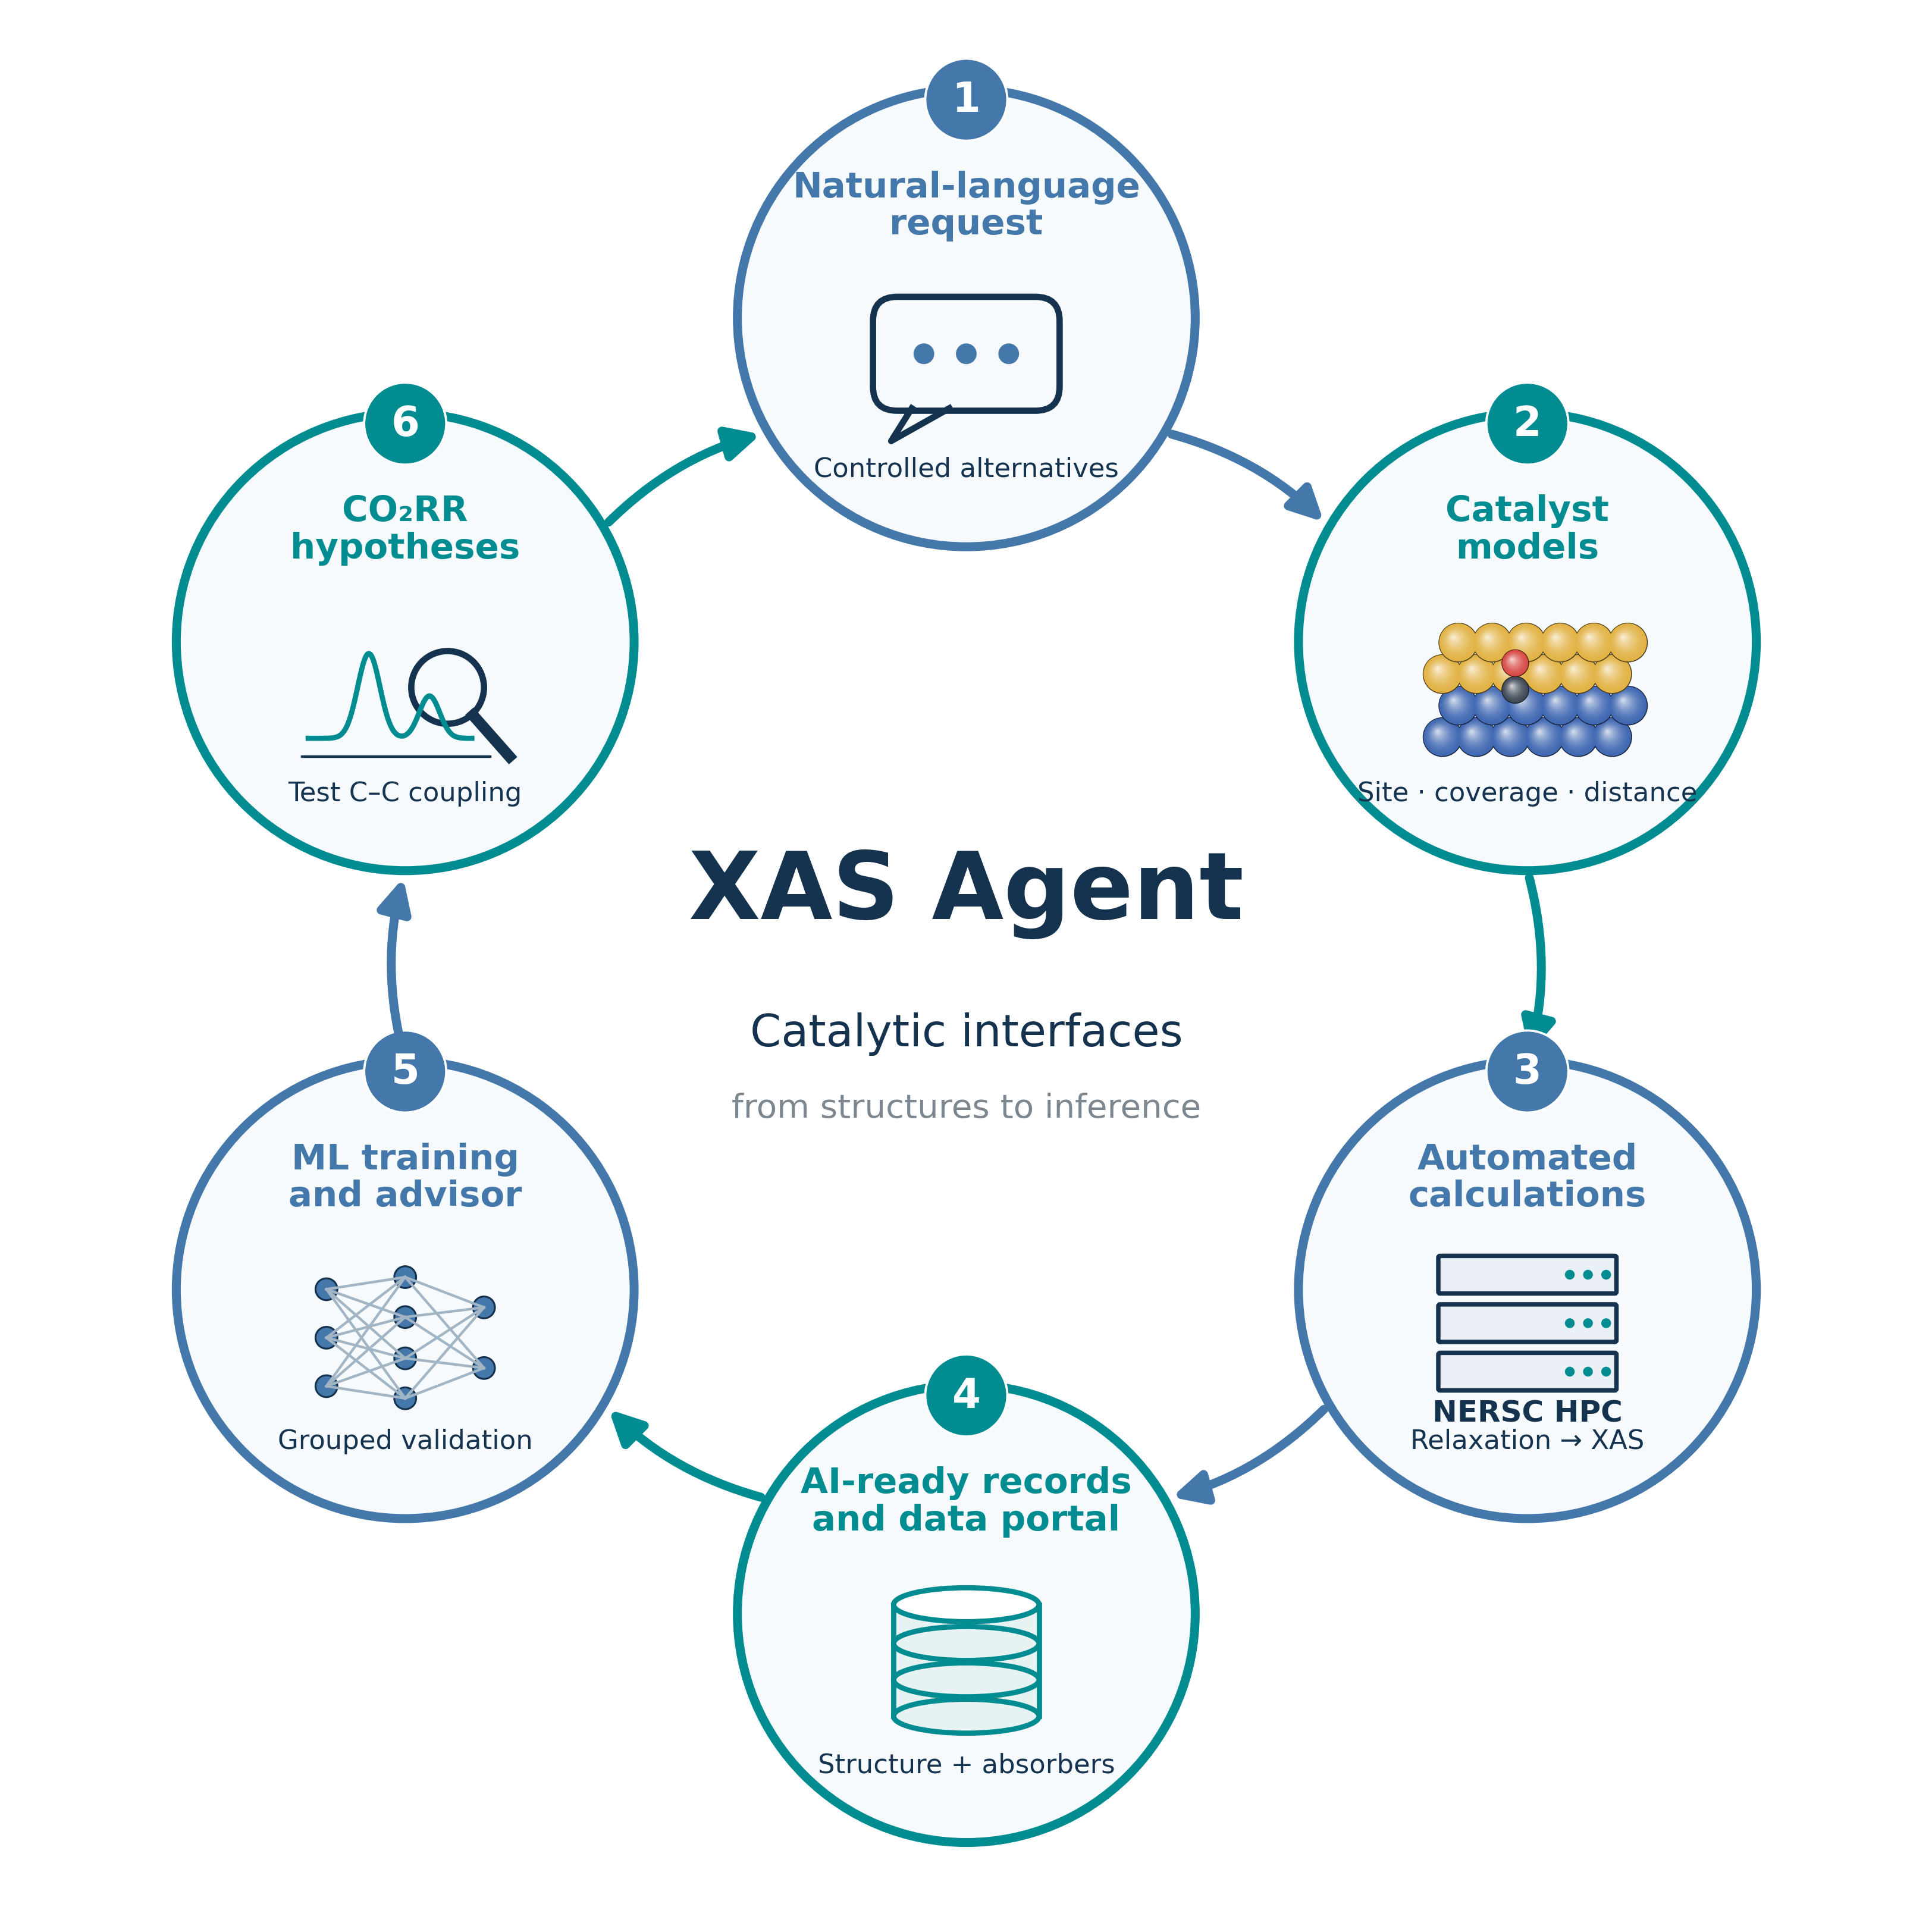
\includegraphics[width=.92\linewidth]{figures/Figure_1_framework.png}
\caption{Hypothesis-driven workflow for catalytic XAS. A scientific request specifies structural alternatives that are generated, relaxed, and evaluated by spectroscopy calculations. The calculation agent manages NERSC execution, and AI-ready records connect the outputs to model training and spectral interpretation. The return arrow represents refinement of the next calculation or hypothesis; it does not imply that a closed-loop catalytic discovery experiment has been completed.}
\label{fig:framework}
\end{figure}

The calculation agent directly manages remote work on the National Energy Research Scientific Computing Center (NERSC) Perlmutter supercomputer. After the user supplies access, allocation, and calculation settings, it can prepare job inputs, transfer files, submit and monitor scheduler jobs, and advance from successful relaxation to XAS. Persistent workflow state supports monitoring and recovery without maintaining an active chat session.\cite{nersc} This design reduces repeated manual file handling and scheduler interaction. Routine transfers, submissions, and monitoring therefore proceed with minimal manual intervention once the workflow is configured, while scientific choices and exceptional failures can be reviewed.

Relaxation is a scientific checkpoint because it determines which chemical state is actually probed. The spectrum is generated from the relaxed geometry, and the resulting record preserves the absorber ensemble and observed adsorbate identity. This prevents a requested OCCO starting model that separates into CO from being interpreted as evidence for a coupled state. The calculation stage and the dedicated analysis interface together cover model generation through predictive evaluation; automatic selection of the next catalytic experiment is a subsequent use of their outputs.

\subsection{Representing interfacial chemical space}
At a bimetallic interface, nominal composition alone cannot identify the environment responsible for a spectral change. CO bound to three Cu atoms and CO bound to one Cu and two Au atoms experience different local coordination even on the same parent surface. Conversely, an all-Cu binding motif can lie either near the boundary or on a Cu terrace. To distinguish these effects, each construction specifies the parent surface, the metal atoms defining the adsorption site, and the adsorbate's distance from the nearest interface (Fig.~\ref{fig:dataset}). Figure~\ref{fig:dataset}a shows the two structural ingredients separately: the Cu--Au substrate interface on the left and the adsorbate models on the right. The extended-surface illustration in Fig.~\ref{fig:dataset}c includes Cu and Au atop sites, Cu--Cu and boundary-spanning Cu--Au bridges, and CuCuCu, CuCuAu, and CuAuAu hollows. These configurations allow changes in local composition to be examined separately from changes in binding multiplicity or interface proximity.

\begin{figure}[!htbp]
\centering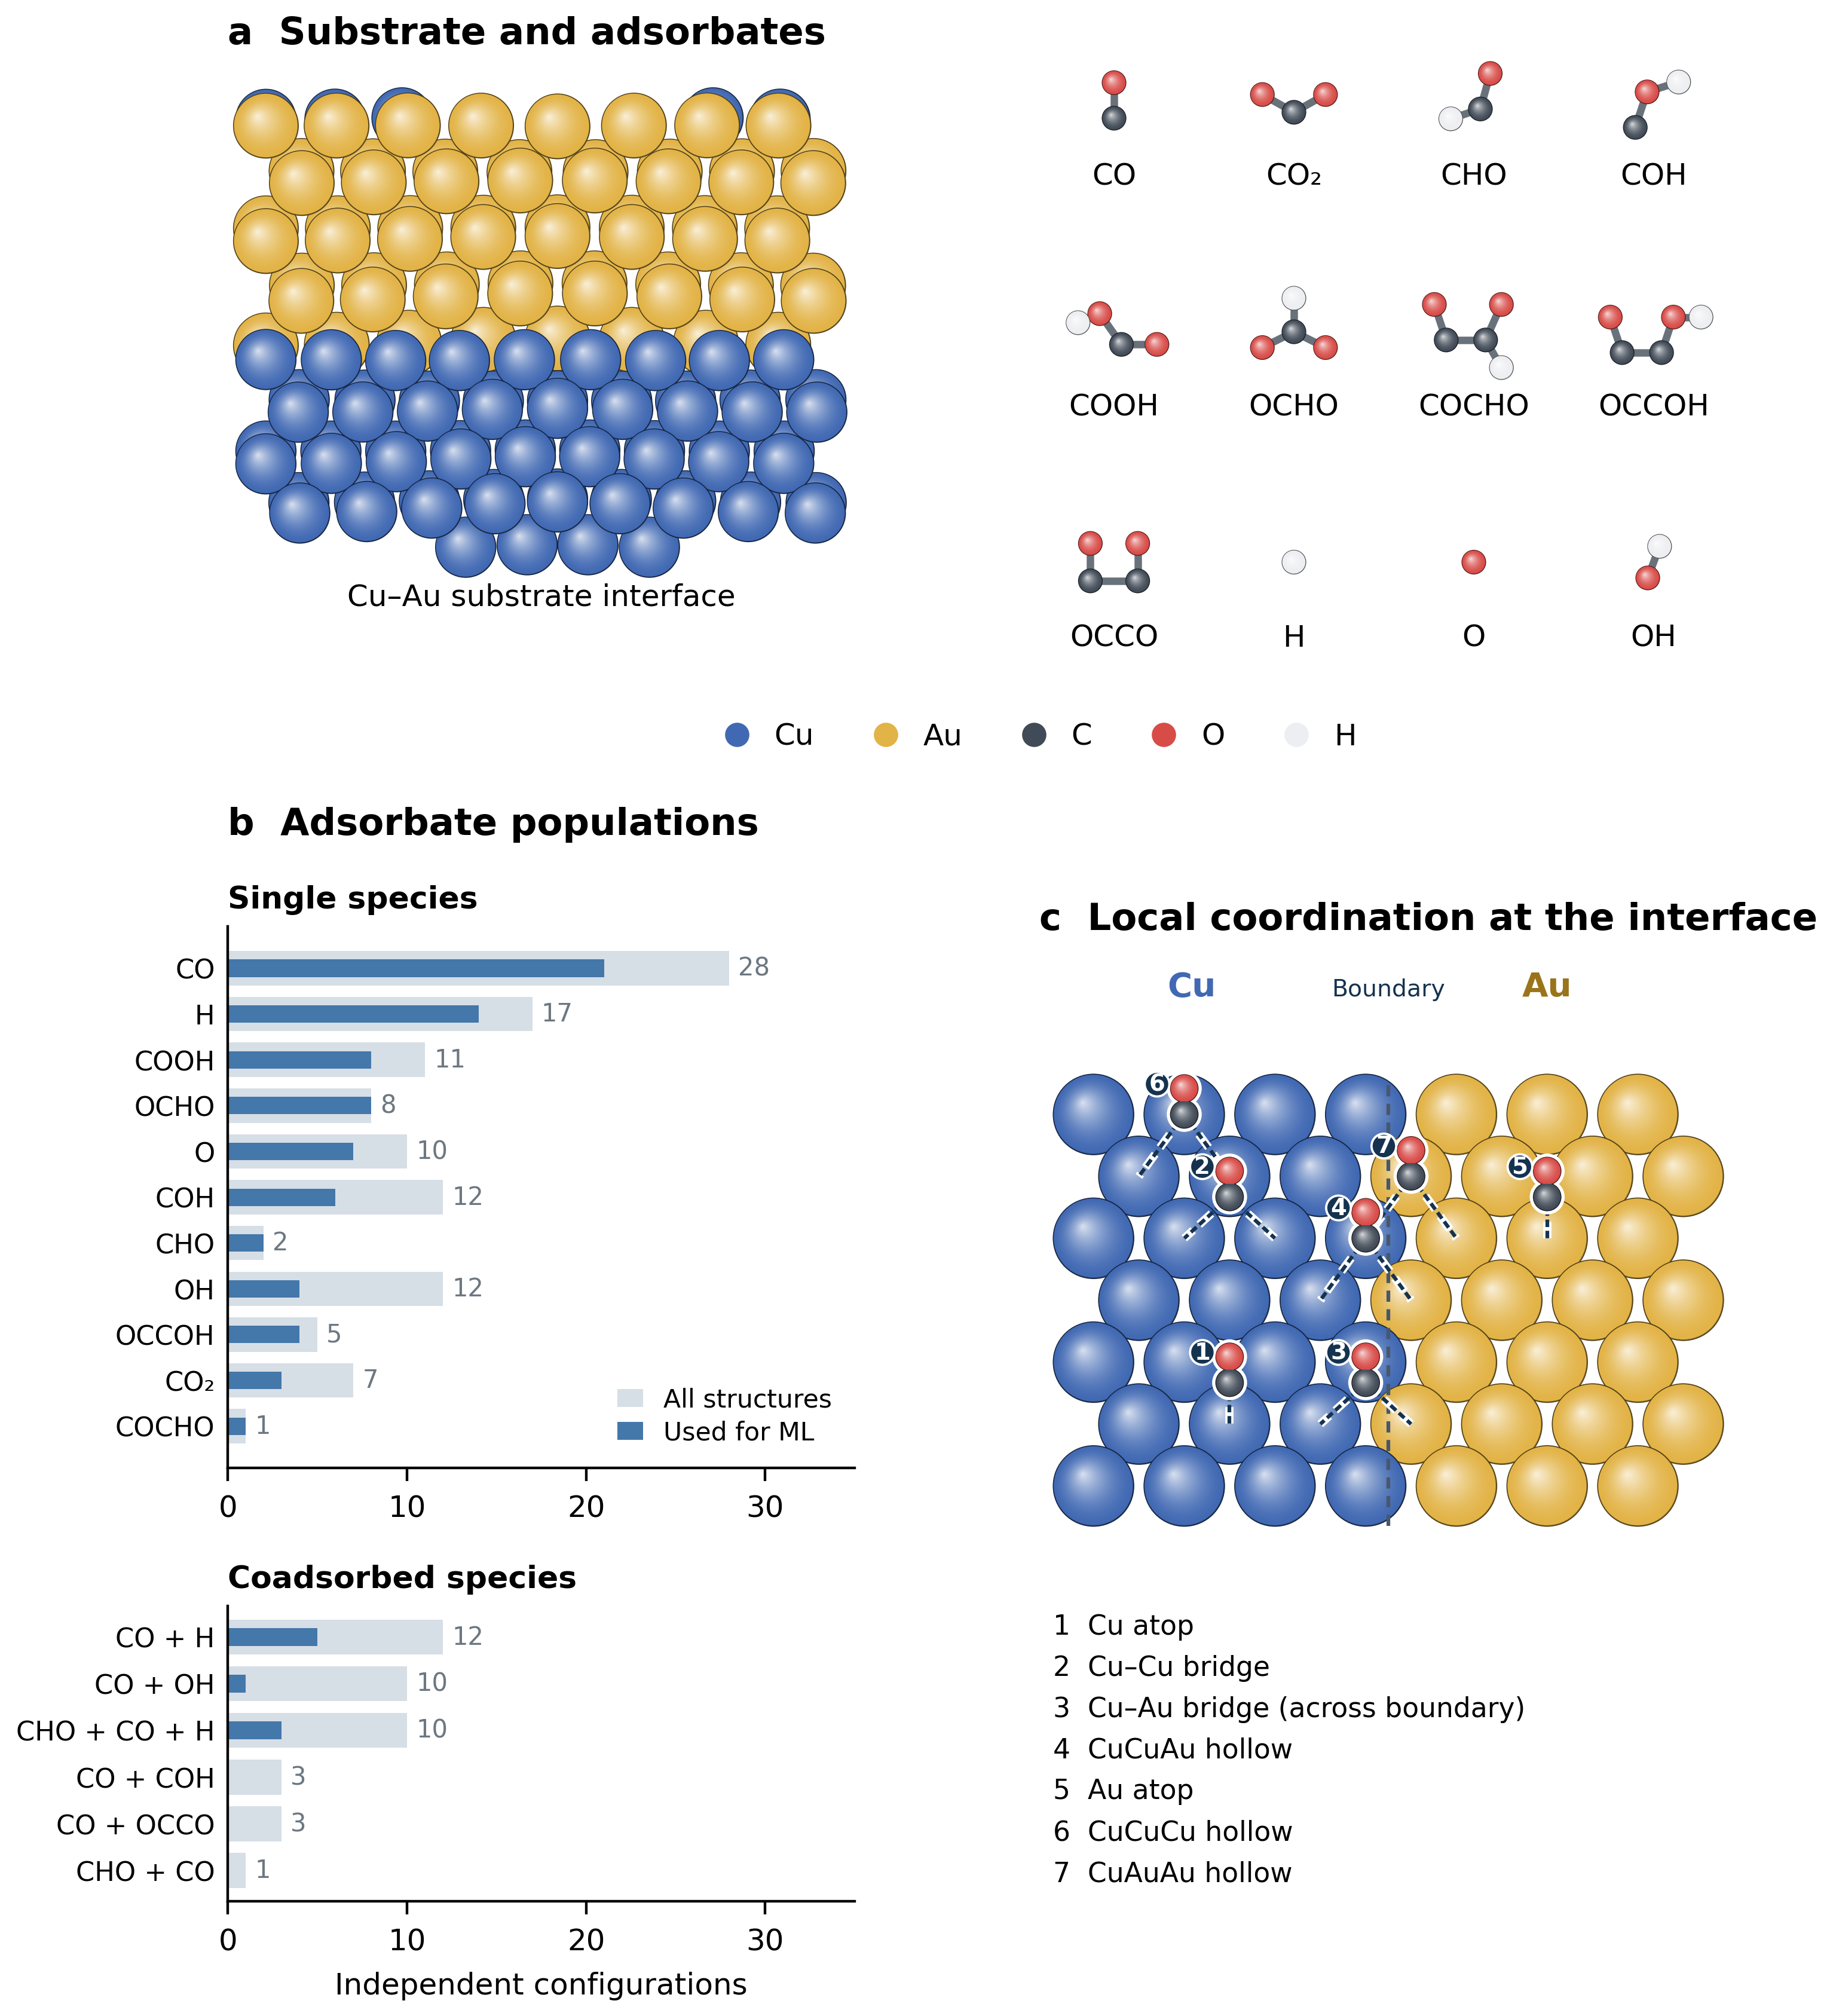
\includegraphics[width=\linewidth]{figures/Figure_2_dataset.png}
\caption{Substrate, adsorbate, and adsorption-site models. (a) Left: the Cu--Au substrate interface rendered from representative input coordinates, showing the two metal regions without adsorbates. Right: schematic structures of the adsorbates considered in the sampling plan. One shared element legend applies to both views: Cu, Au, C, O, and H are blue, gold, dark gray, red, and light gray. (b) Archived exclusive configuration counts (152 adsorbate-bearing inventory structures and 87 ML configurations: 78 single-species and 9 mixed), separated into single-species and coadsorbed states, for the full inventory and completed ML dataset. A single-species state can contain several molecules of that species. Two clean surfaces and one CuO reference are omitted from these adsorbate counts. (c) Seven CO adsorption motifs on one schematic Cu--Au surface, with adsorbates and metal atoms in the same oblique projection. Numbered sites and dashed contact lines define atop, bridge, and hollow coordination, including the boundary-spanning bridge and three hollow compositions. These site illustrations are not relaxed structures.}
\label{fig:dataset}
\end{figure}

The Cu--Au construction space includes pure Cu(111) and Au(111) surfaces and lateral stripe ratios of 1:1, 2:1, 1:2, 3:1, and 1:3. Explicit row counts define the parent model, while adsorption positions distinguish boundary, neighboring-row, and terrace environments. These are the available structural controls; the completed cohort samples a subset of their combinations. At each location, coverage and spatial distribution determine how many metal environments are perturbed and whether adsorbates have nearby reaction partners. Molecular coverage is therefore retained together with its reference surface population. Carbon-equivalent coverage provides an additional comparison for OCCO and spectator CO, permitting equal carbon loading to be maintained when two CO molecules form one coupled intermediate.

Equal loading does not, however, imply equal chemical identity. Neighboring CO molecules remain an uncoupled state unless a C--C bond forms; separate CO and H likewise differ from bonded CHO. Molecular connectivity and metal contacts are checked after relaxation so that the spectral label describes the state actually calculated. Single-species and coadsorbed configurations are distinguished in Fig.~\ref{fig:dataset}b. Together, these controls make the dataset suitable for asking which spectral differences arise from chemistry and which arise from changes in the surrounding interface.

\subsection{Preserving the information needed for a hypothesis test}
The records carry the information needed to decide whether two spectra constitute a controlled comparison. Adsorbate identity and molecular count specify the chemical alternatives; local coordination, interface distance, and coverage identify possible confounding changes. Absorber populations and calculation settings define how those structures contribute to the computed signal. Retaining these quantities together allows spectra to be regrouped for a new question without reconstructing their meaning from filenames. Coadsorption is treated as simultaneous species presence: CO+H contains two labels, while bonded CHO is a distinct molecular label. Structural descriptors define targets and support quality control; the classifiers reported here receive spectral features only.

A second hypothesis concerns observability: a real intermediate can be spectroscopically difficult to detect if most absorbers are far from it. Layer-resolved spectra separate this dilution question from changes in adsorbate identity. They permit surface and subsurface contributions to be examined for the same configuration. For layer means $\mu_l(E)$ representing $n_l$ Cu sites, a combined representation is formed as
\begin{equation}
\mu_D(E)=\frac{\sum_{l\in D}n_l\mu_l(E)}{\sum_{l\in D}n_l}.
\label{eq:average}
\end{equation}
Population weighting precedes spectral normalization. This preserves the physical meaning of a layer average and avoids assigning equal contributions to ensembles containing different numbers of absorbers. The same configuration is then evaluated through individual-layer and combined-layer representations, allowing depth sensitivity to be compared without changing the underlying sample population.


\section{Results and discussion}
\subsection{Reference-material comparison and a practical calculation route}
Cu, Cu$_2$O and CuO test spectral shape and identify limitations of the calculation route (Fig.~\ref{fig:reference}). Formal Cu(0), Cu(I) and Cu(II) labels describe the reference compounds; they are not inferred continuous atomic charges. Fourteen of the fifteen computational material/method slots have numeric spectra. Current Cu$_2$O PBE and GW-labelled outputs supply previously missing arrays; the supplied CuO PBE output still lacks a recoverable complete numeric XAS table. Missing slots are retained explicitly.

The VASP curves use the diagonal-tensor average and the notebook's additional Gaussian $\sigma=1$ eV (FWHM 2.35482 eV), retaining native broadening. No universal extra Lorentzian is imposed. The Cu$_2$O inputs specify PBE+$U$ with $U_{\mathrm{eff}}=6$ eV on Cu. GW-labelled PAW datasets and IALGO do not establish a quasiparticle GW or Bethe--Salpeter calculation. These curves are therefore distinguished by their supplied dataset labels, with the actual electronic stages documented in the SI. FDMNES and FEFF final spectra are not convolved twice.

Every reference overlay and similarity score uses the same min--max rule on the identical 8980--9015 eV grid: $(I-I_{\min})/(I_{\max}-I_{\min})$. The displayed Cu$_2$O axis remains 8975--9015 eV; unsupported pre-window values are not extrapolated. An unsupported local pre-edge subtraction that introduced negative CuO finite-difference intensity is removed. Raw data and stage-by-stage diagnostics remain available. This relative-intensity comparison does not establish absolute cross-section accuracy.

\begin{figure}[!htbp]\centering
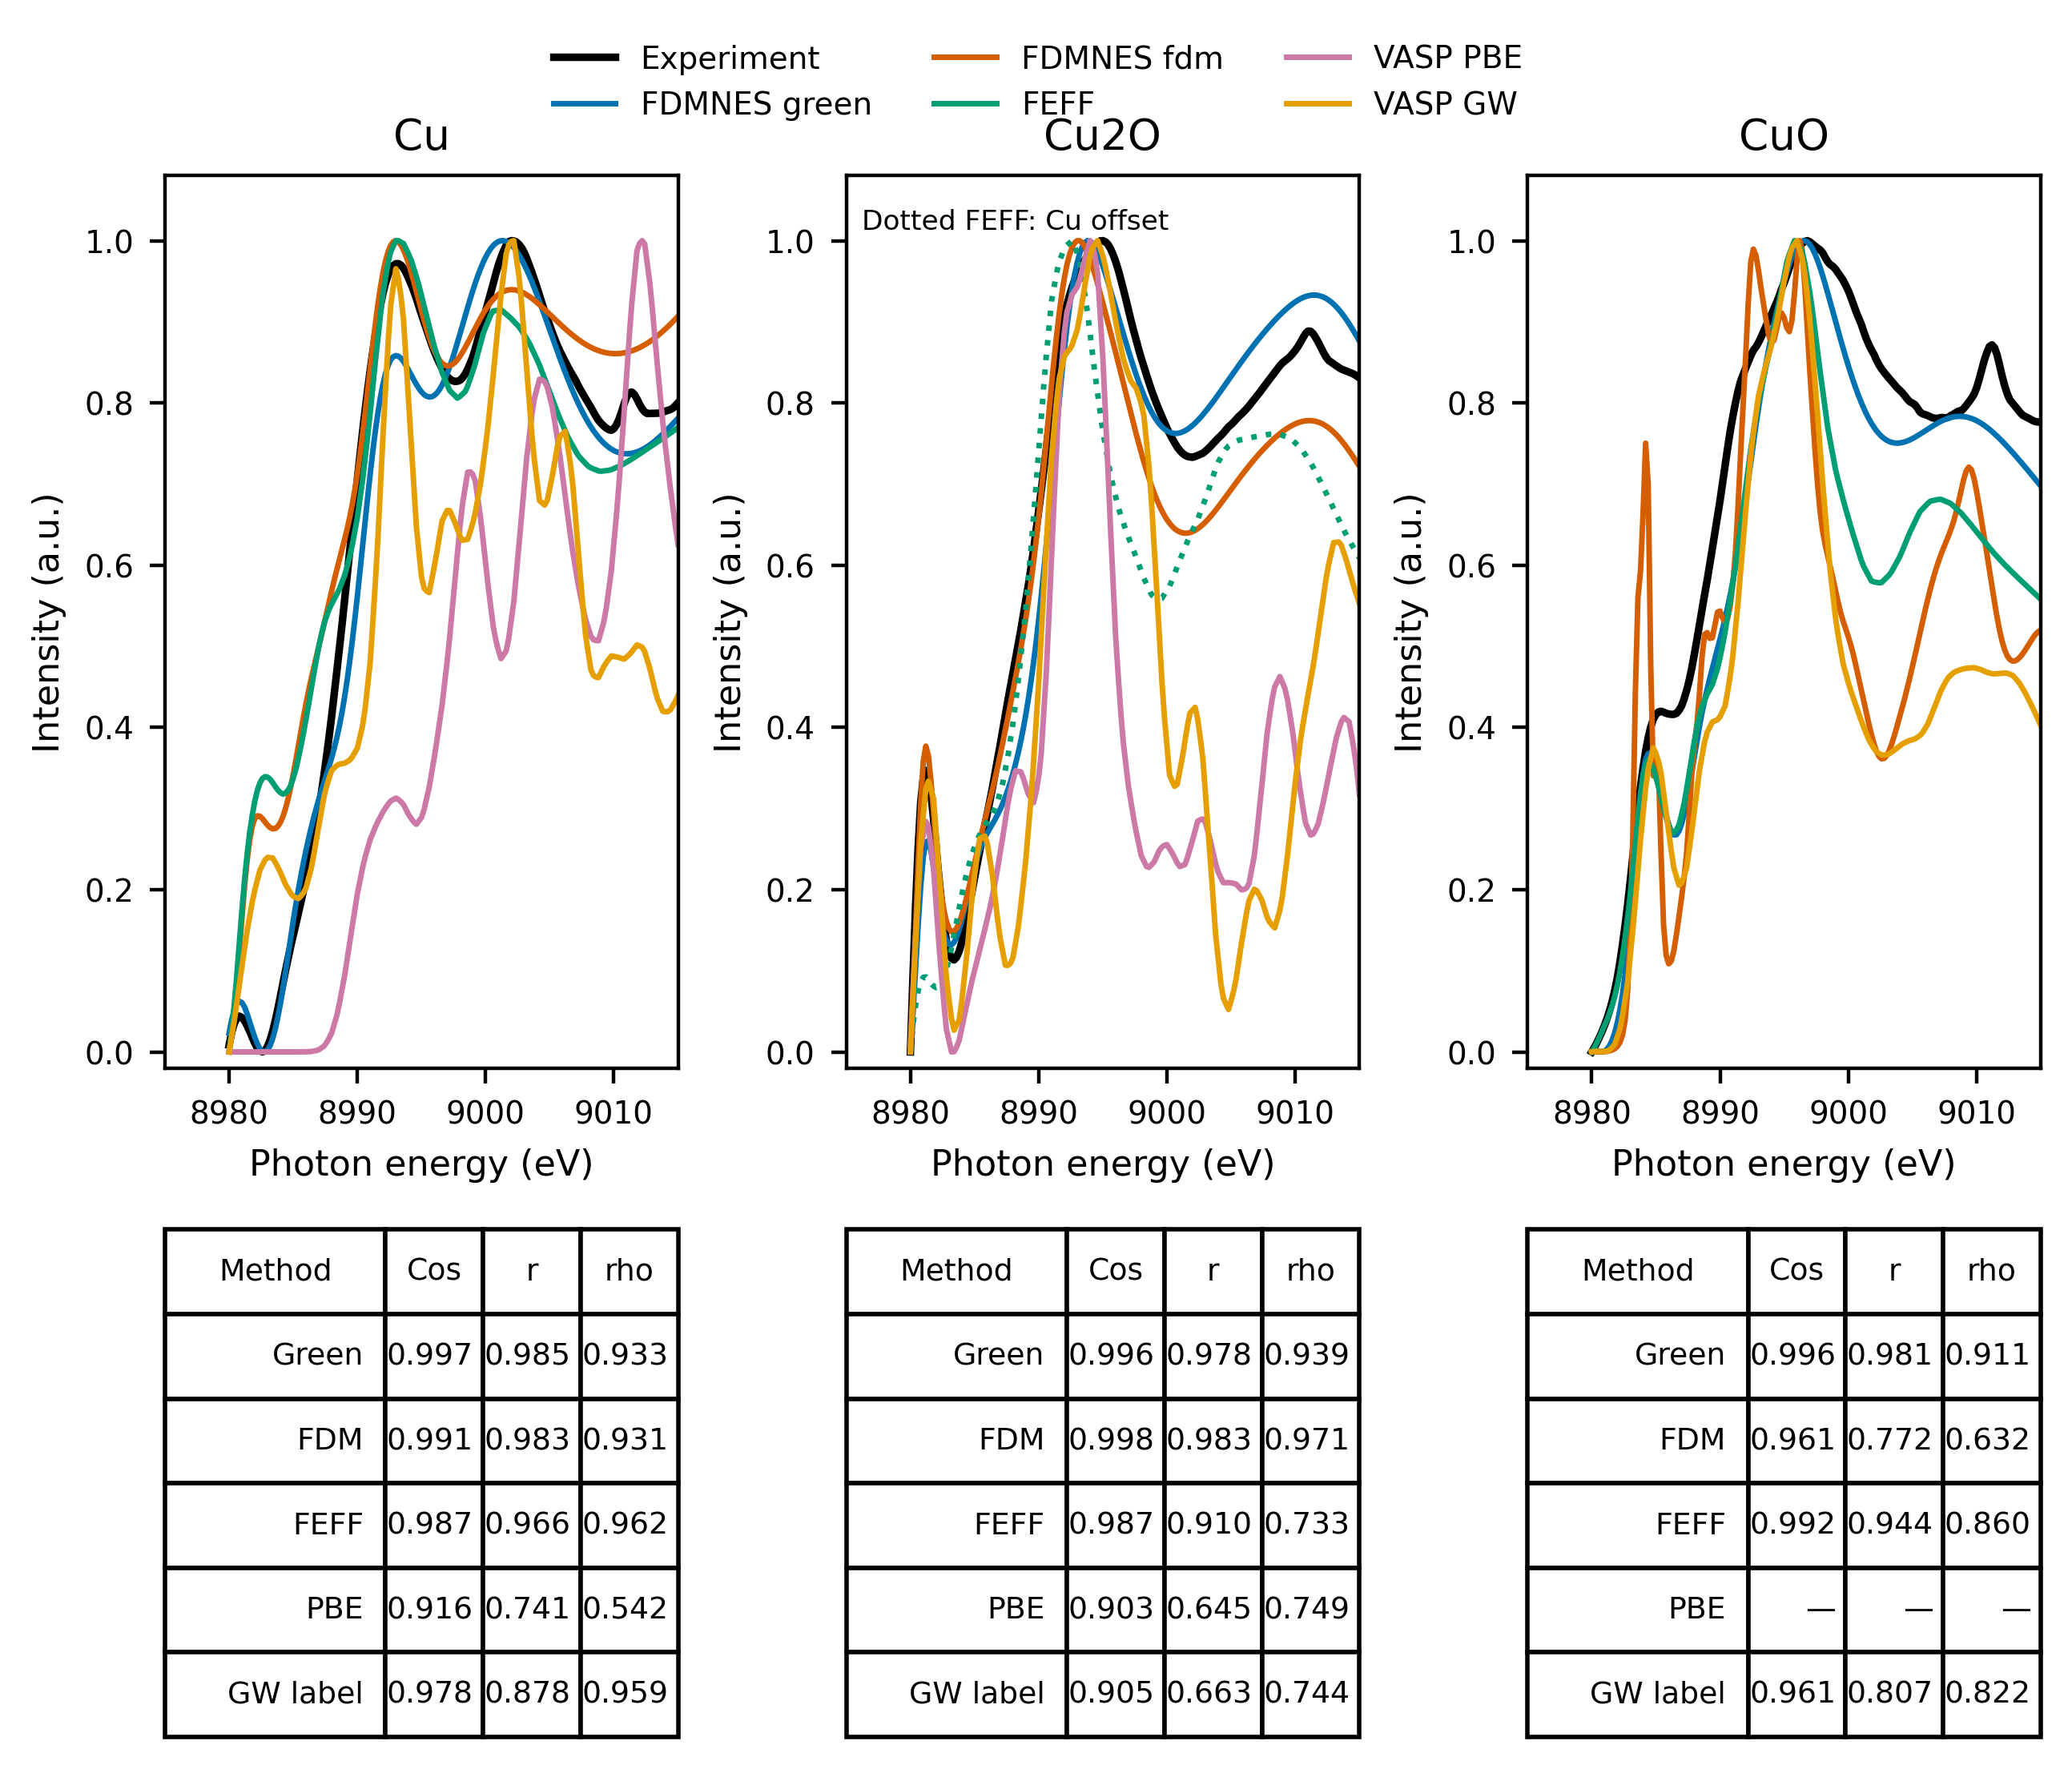
\includegraphics[width=\linewidth]{figures/reference_comparison.png}
\caption{Numeric Cu/Cu$_2$O/CuO reference comparison. Scores immediately beneath each spectrum are cosine similarity, Pearson $r$ and Spearman $\rho$ on the plotted normalized arrays. The first-feature-aligned view diagnoses shape; separate Cu-calibrated transferable offsets are reported in the SI. Cu$_2$O uses its early peak at 8981.29 eV, while CuO uses the early rising inflection at 8983.29 eV. The dotted Cu$_2$O FEFF trace retains its Cu calibration because an early feature is unresolved; its legend states this exception. Missing CuO PBE remains blank. Independently aligned compounds do not test absolute chemical-shift agreement.}\label{fig:reference}
\end{figure}

In the shape comparison, Green-function FDMNES gives Pearson correlations of 0.985, 0.978 and 0.981 for Cu, Cu$_2$O and CuO. Finite differences slightly improve Cu$_2$O (0.983), whereas their CuO agreement is poorer (0.772). FEFF and the GW-labelled Cu calculation have stronger rank correlation than Green for Cu despite lower Pearson agreement. No single metric supports a universal winner. Green therefore remains a practical survey route for the broad configuration space, supported by these reference shapes and its documented economical multiple-scattering formulation,\cite{joly2001,fdmnesmanual} with transfer limitations rather than a measured speedup. Unequal native final-state treatments and incomplete timing comparability preclude a controlled cost--accuracy ranking.

\subsection{From source weights to physically scaled pairs}
A source-level audit is necessary before subtracting spectra. The clean Cu--Au layers contain 36 physical Cu atoms each, but their recorded symmetry multiplicities sum to 51 and 52. Repeating the native convolution from the saved raw site spectra and decks reproduces all 232 audited top-layer outputs. For source lists already covering every physical atom, each symmetry-summed source is weighted by its inverse multiplicity before dividing by the physical Cu population. The clean correction is energy dependent; dividing the aggregate by a guessed scalar would not reproduce it. Corrected records are versioned separately from the archived benchmark. This reconvolution reuses completed electronic spectra and introduces no new electronic calculations.

Thirty-four adsorbed Cu--Au configurations share the clean model's initial metal coordinates, cell and constraints. These are primary matched-model pairs, not independently proven historical parent lineages. Sixty-four additional same-substrate cases form a weaker sensitivity set. Their relaxed metal coordinates may change through adsorption; this physical response is retained. The reference is an actual separately relaxed clean interface, not a species-absent ensemble or a frozen covered slab with molecules removed. Seventeen Cu(100) configurations lack a located compatible completed clean spectrum, so joint differential training is not claimed. Compatible clean relaxation/XAS inputs are prepared without submission.

For physical layer means $\mu_l$ in Mbarn per Cu, Eq.~\ref{eq:average} combines the same physical top two layers in each member. Cu--Au uses layers 4+5; Cu(100) would require 3+4. Missing top layers cannot be replaced by deeper ones. On the common 8974--9029 eV grid,
\begin{equation}
 d_i(E)=\frac{\mu_{\mathrm{ads},i}(E)-\mu_{\mathrm{clean},p(i)}(E)}{S_{p(i)}},\quad
 S_p=\langle\mu_{\mathrm{clean},p}\rangle_{9018:9025}-\langle\mu_{\mathrm{clean},p}\rangle_{8974:8977}.
\label{eq:delta}
\end{equation}
The clean-derived divisor is shared by the pair. Both signs and amplitude are retained; there is no per-difference minimum subtraction, area, peak or norm normalization, and no independent alignment of pair members. This spectral contrast includes adsorption-induced substrate relaxation. It does not isolate one species within a mixture.

\subsection{Matched identity and CO-loading tests}
Five configuration-held-out folds and three inner grouped folds compare five representations: archived-method normalized raw, source-corrected normalized raw, physically scaled raw, signed $d$, and $[\mu_{\mathrm{clean}}/S,d]$. Every comparison uses the same eligible configurations and targets. Inner training selects compact Combined or DCT8/16/24 features and regularization, as well as identity thresholds. Featurewise scaling is fitted only on training data. Signed cumulative differences are integrals of $d$, not probability CDFs; their values can decrease. DCT dimensions include the constant coefficient.\cite{ahmed1974} Molecular counts, site labels, filenames and structural metadata never enter the spectral predictors.

\begin{figure}[!htbp]\centering
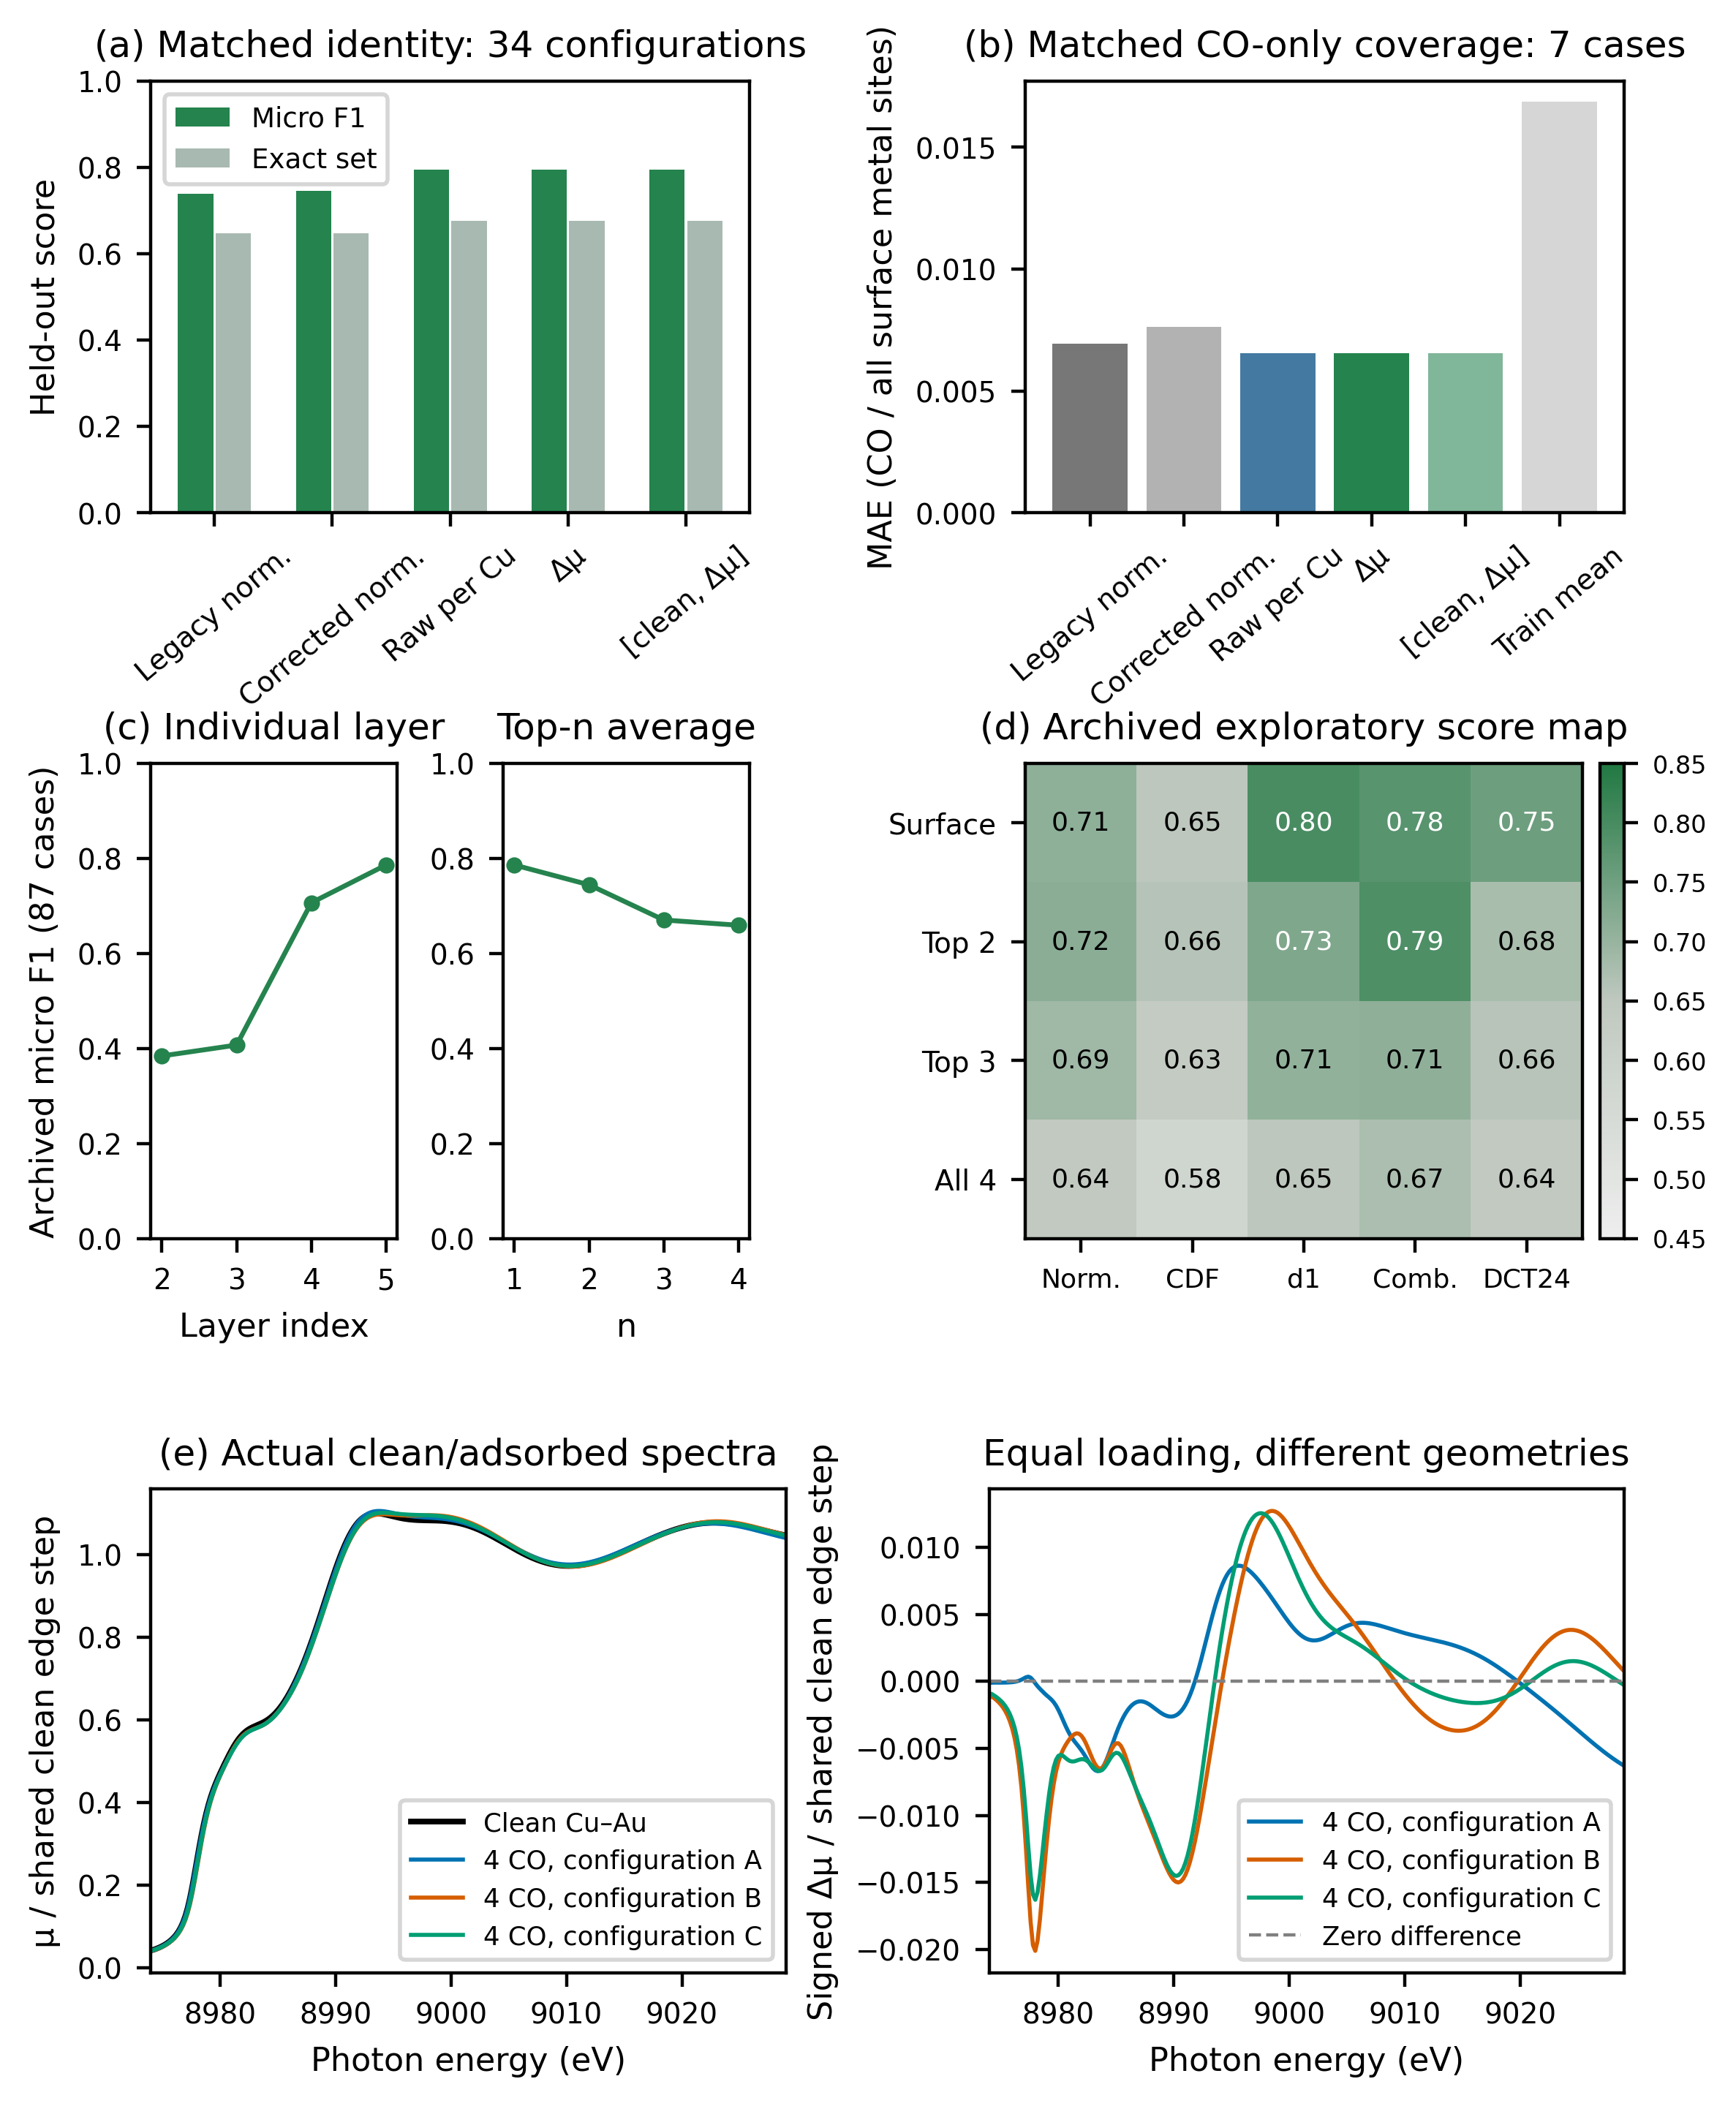
\includegraphics[width=\linewidth]{figures/Figure_4_differential_ML.png}
\caption{Matched-cohort comparison and actual clean-reference contrasts. (a) Identity, 34 independent configurations. (b) CO-only loading, seven configurations; the denominator is all 68 surface metal sites. (c) Archived 87-configuration individual-layer and top-$n$ averages are shown separately. (d) Archived exploratory feature/depth score map, retaining its green-to-gray scale; it does not select the new study's method. (e) Native clean and adsorbed per-Cu spectra and signed differences share one clean-derived scale. Three four-CO configurations illustrate geometry/distribution changes at equal loading, rather than a species-specific response. The dashed gray line denotes zero difference. Exact identities and paired arrays are supplied.}\label{fig:ml}
\end{figure}

\textit{Normalized energy spectrum} means intensity sampled on the fixed energy grid after the archived minimum-subtracted unit-area transformation; the energy axis itself is not normalized. CDF is the cumulative integral of that nonnegative normalized raw spectrum, d1 its first energy derivative, and Combined its smoothed spectrum, integral and first/second derivatives. These archived features are distinct from the signed differential definitions.

The 34-case primary subset contains six supported labels (CO, H, O, COH, COOH and OH). Legacy normalized raw gives micro F1 0.7385 and exact-set accuracy 0.6471; source-corrected normalized raw gives 0.7463 and 0.6471. Physically scaled raw, $d$, and the paired representation each give 0.7941 and 0.6765. Macro F1 is 0.3635 across all eleven declared labels, or 0.6665 across the six supported labels. These denominators are reported separately. The conditional paired 95\% interval for the micro-F1 difference between $d$ and corrected normalized raw spans $-0.0195$ to $0.1205$; it resamples fixed held-out predictions, not refitted models or independent parent families.

For the seven matched CO-only configurations, the target is $\theta_{\mathrm{metal}}=N_{\mathrm{CO}}/N_{\mathrm{surface\ metal}}$. The physically scaled raw, $d$, and paired models all give MAE 0.00655 and $R^2=0.714$. Legacy and corrected normalized controls give MAE 0.00695 and 0.00763. The difference against legacy normalization has a conditional interval crossing zero. The Cu-normalized loading $N_{\mathrm{CO}}/N_{\mathrm{surface\ Cu}}$ is a distinct target (MAE 0.01236 here), related by $\theta_{\mathrm{metal}}=(36/68)\theta_{\mathrm{Cu}}$. It is not literal Cu-site occupancy, because CO may contact Au or multiple metals. Areal density in CO/nm$^2$ is also retained as a separate structural target. CO-containing mixtures are not counted as additional CO-only regression cases.

An explicit mixture diagnostic applies the mean of the five saved CO-only fold models to four matched CO-containing mixture configurations, absent from every model fit and selection. Physical raw and differential MAE is 0.02021 CO/all surface metal sites, with $R^2=-10.31$. Thus the CO-only predictor does not establish mixture coverage inference; coadsorbates change the spectral response. This frozen-model diagnostic is distinct from mixture-trained cross-validation.

Subtraction adds no accuracy over amplitude-preserving raw spectra in this study. A fixed reference is an affine translation; after training-only centering, it adds no independent information to the linear control. Constant reference columns are removed using training data. This result supports an auditable difference observable without demonstrating substrate invariance or a new predictive advantage. One shared clean-model family cannot establish leave-parent-out generalization.

Local geometry is evaluated separately from identity and loading. All seven primary CO configurations have the same atop-like Cu-contact target, making zero contact error trivial. The broader 25-case CO sensitivity set supplies contact diversity, but the CO hollow-molecule support is Cu$_3$/Cu$_2$Au/CuAu$_2$/Au$_3$ = 25/2/0/0. Molecules are not independent spectral samples. Cu(100) supplies genuine atop/bridge examples, not missing Au-rich hollows; inference across all four hollow compositions remains unsupported.

\subsection{Cu(100) augmentation, robustness and experimental limits}
Without a compatible clean Cu(100) spectrum, only raw-input controls can evaluate its current contribution. A fixed DCT16/Ridge($\alpha=10$) control reproduces Cu-normalized loading MAE 0.082124 with Cu--Au-only training and 0.035186 when each of four Cu(100) cases is held out while the other three enter training. Identical Cu--Au folds change from 0.027756 to 0.026766. Loading and motif vary together in only four Cu(100) cases. A separate four-label raw identity control on 12 supported Cu(100) cases changes micro F1 from 0.4375 to 0.6429 with other Cu(100) training cases; five H$_2$O/CO$_3$ cases remain unsupported-chemistry tests. These exploratory conditional-configuration results establish neither differential transfer nor independent facet validation.

\begin{figure}[!htbp]\centering
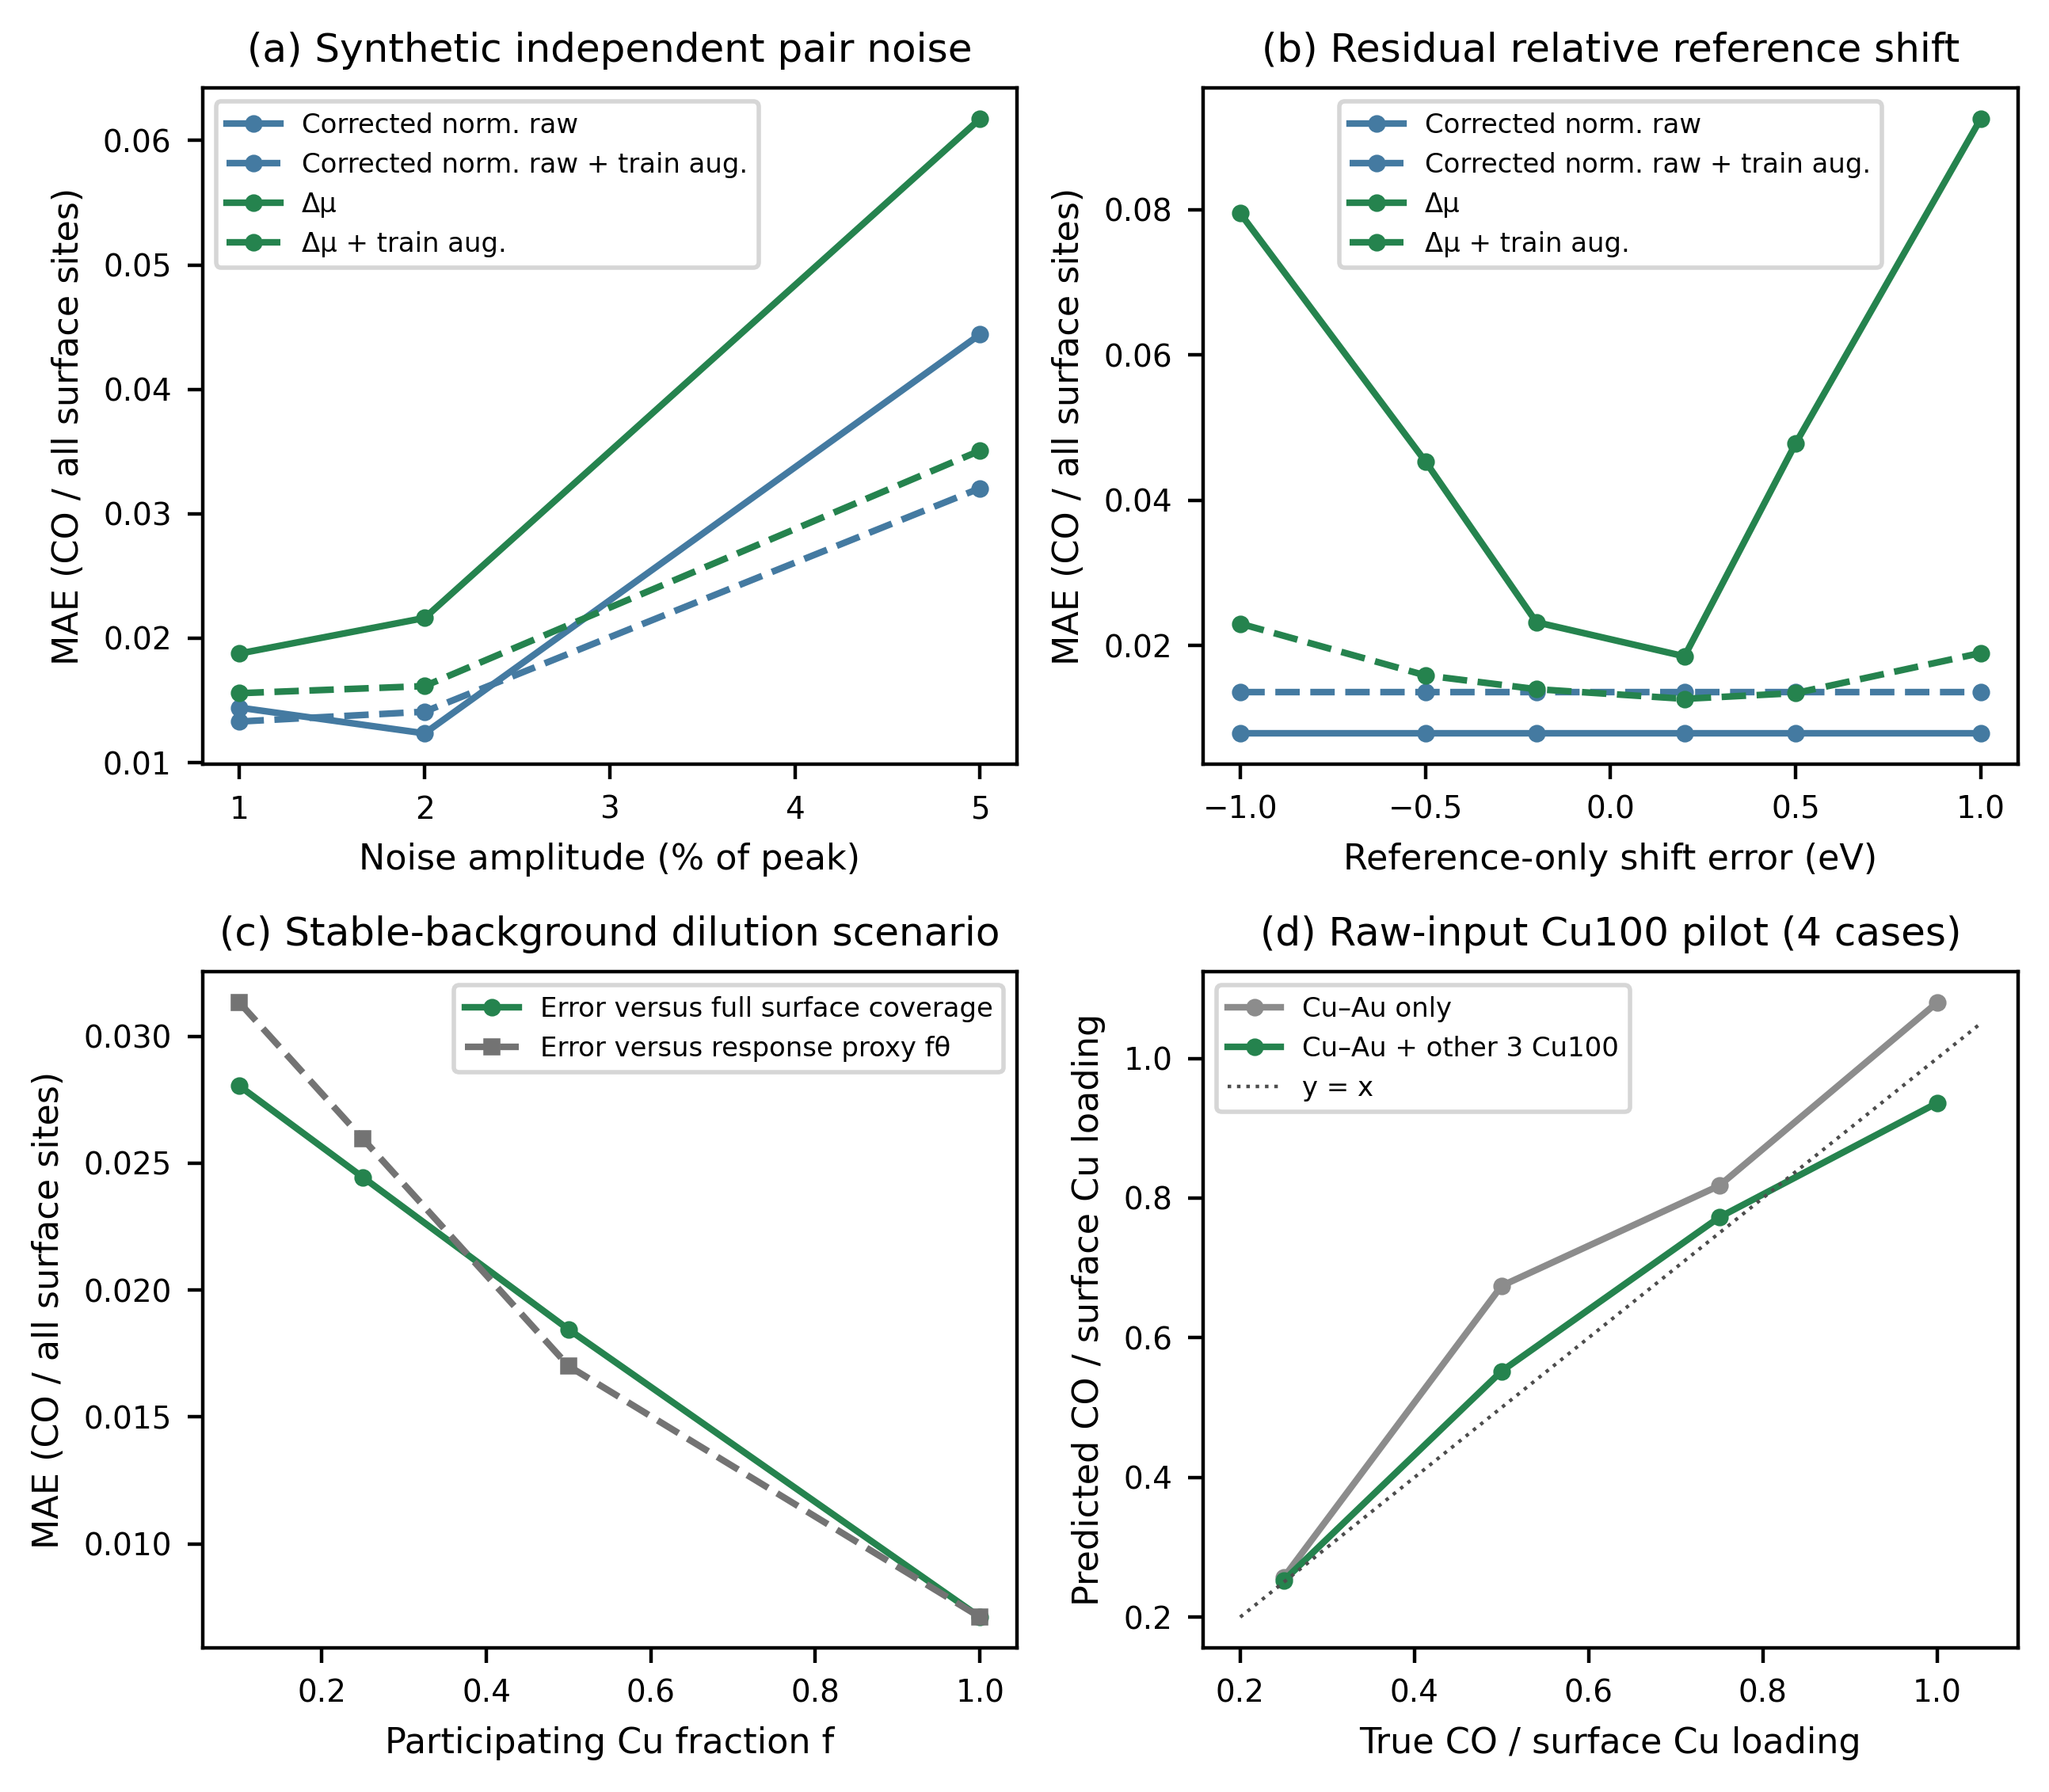
\includegraphics[width=\linewidth]{figures/Figure_5_robustness_transfer.png}
\caption{Declared synthetic stress tests and a separate raw-input augmentation control. (a,b) Independent paired noise and residual relative reference-energy error, applied before subtraction; dashed curves use training-only augmentation. (c) Stable-background dilution $\mu_{\mathrm{obs}}=\mu_{\mathrm{clean}}+f(\mu_{\mathrm{ads}}-\mu_{\mathrm{clean}})$ distinguishes error against full surface loading from an $f\theta$ response proxy. Subtraction cannot determine $f$. (d) Raw-spectrum Cu(100) loading predictions from four leave-configuration-out cases. These are simulated scenarios and exploratory controls, not measured instrumental uncertainty or experimental validation.}\label{fig:robustness}
\end{figure}

The fixed robustness protocol evaluates common and residual energy shifts, gain/edge-step error, extra Gaussian broadening, independent and shared-reference noise, and surface fractions 0.1--1. Arrays are cropped to 8976--9027 eV so every trial has full support. Native lifetime broadening is preserved. All augmented views remain with their parent configuration; outer tests do not select nuisance settings. Subtraction can cancel a stable substrate background while increasing independent noise and sensitivity to a misregistered reference. Shared-reference noise also couples errors between configurations. The complete scenario table therefore accompanies clean performance rather than selecting a favorable condition.

Experimental use requires a compatible paired reference measured on the same catalyst or a validated equivalent state, with documented incident intensity, thickness/concentration, self-absorption, detection geometry and energy calibration. Operando oxidation, morphology, potential and solvent changes can also contribute to $\Delta\mu$. Residual reference adsorbates change the target to a change relative to that state. The illuminated surface fraction must be independently constrained before a slab-normalized response can be interpreted as absolute surface coverage. Established difference-XANES sensitivity motivates this route,\cite{ramaker2010,ramaker2014} but no labeled paired experimental validation is available here.

\subsection{Archived benchmark and the shared agent route}
The historical benchmark remains unchanged: 87 independent configurations, 348 layer spectra, primary micro/macro F1 0.7791/0.6383 and exact-set accuracy 0.6897. The exploratory fixed winner remains 0.7978/0.6597 and 0.7011. Saved primary and fixed-winner arrays match the recorded fresh run; 140 of 169 broader OOF files match and 29 variants differ. Dependency versions differ, but causation needs a controlled version experiment. All five recorded fold-model reload checks match. These are archived run records, distinct from current paired-study checks. In the primary saved predictions H is recovered in 14/14 single-species cases but 0/8 mixtures; CO is recovered in 21/21 single-species cases and 5/9 mixtures. A single-species bar counts configurations, not molecules or all positives.

The paired workflow is exposed through the same audited scientific callable used by the agent and interface. A local natural-language request validates pairs, fits declared recipes, saves and reloads models, and predicts genuinely held-out records. Reference identities, physical populations, units and transformation provenance accompany each model. Reference-free or incompatible-domain differential queries fail explicitly. Experimental requests require a declared paired preprocessing and population convention and remain flagged as unvalidated transfer. This local demonstration does not establish production scheduler execution or newly generated spectra.

\section{Outlook: controlled coupling and additional references}
The matched adjacent-CO/OCCO comparison requires verified relaxed connectivity and compatible completed spectra, not equal formulas alone. The current three water-containing relaxation checkpoints are dissociated 2CO: C--C distances are approximately 3.28, 3.10 and 3.48~\AA, with short C--O bonds and no covalent proton transfer to the original dimer. Their latest CONTCAR geometries define the current identities. Initial coupled seeds do not override this observation. The runs are unfinished and are not established minima or thermodynamic conclusions. Other water/K/reversed/C,O-bound alternatives are available as seeds only. No unfinished checkpoint enters XAS training.

A valid completed Cu K-edge coupled/uncoupled pair would support a scoped chemical contrast; a full interface/terrace quartet would test the difference between those contrasts. Additional C/O edges are extensions, not prerequisites. The next informative controls are the compatible clean Cu(100) reference, independent interface CO and hydrogenated environments, and matched CO/CO+H/CO+OH configurations. Proposed calculations have not already improved the model. Prospective configurations should be locked before inspection for genuinely new confirmation.

\section{Conclusions}
The agent connects catalytic alternatives to geometry-checked spectral records and reproducible inference. A source-resolved convolution audit enables physical per-Cu clean-parent differences without altering the frozen raw benchmark. On the matched Cu--Au cohort, preserving amplitude improves some point estimates relative to normalized controls, but subtraction itself adds no accuracy beyond the same physically scaled raw input. Sparse CO-loading and local-environment support, a missing clean Cu(100) reference and one shared clean-model family limit transfer claims. The resulting paired route is a testable bridge toward measured catalyst/reference differences, with experimental validation and independent parent transfer still outstanding.

\section*{Data and code availability}
Versioned source packages, corrected records, paired arrays, fold assignments, saved recipes/models, held-out predictions, figure code and numerical benchmark stages accompany this article in the study repository. Archived studies are retained separately.
\section*{Acknowledgements}
This work used resources of the Center for Nanoscale Materials, a U.S. Department of Energy Office of Science User Facility at Argonne National Laboratory.
\begin{thebibliography}{99}
\bibitem{ni2024} W. Ni, H. Chen, N. Tang \textit{et al.}, High-purity ethylene production via indirect carbon dioxide electrochemical reduction, \textit{Nat. Commun.}, 2024, \textbf{15}, 6078, DOI: \href{https://doi.org/10.1038/s41467-024-50522-7}{10.1038/s41467-024-50522-7}.
\bibitem{francis2018} S. A. Francis, J. M. Velazquez, I. M. Ferrer, D. A. Torelli, D. Guevarra, M. T. McDowell, K. Sun, X. Zhou, F. H. Saadi, J. John, M. H. Richter, F. P. Hyler, K. M. Papadantonakis, B. S. Brunschwig and N. S. Lewis, Reduction of aqueous CO\textsubscript{2} to 1-propanol at MoS\textsubscript{2} electrodes, \textit{Chem. Mater.}, 2018, \textbf{30}, 4902--4908, DOI: \href{https://doi.org/10.1021/acs.chemmater.7b04428}{10.1021/acs.chemmater.7b04428}.
\bibitem{zhan2024} C. Zhan, F. Dattila, C. Rettenmaier, A. Herzog, M. Herran, T. Wagner, F. Scholten, A. Bergmann, N. L\'opez and B. Roldan Cuenya, Key intermediates and Cu active sites for CO\textsubscript{2} electroreduction to ethylene and ethanol, \textit{Nat. Energy}, 2024, \textbf{9}, 1485--1496, DOI: \href{https://doi.org/10.1038/s41560-024-01633-4}{10.1038/s41560-024-01633-4}.
\bibitem{montoya2015} J. H. Montoya, C. Shi, K. Chan and J. K. N\o rskov, Theoretical insights into a CO dimerization mechanism in CO\textsubscript{2} electroreduction, \textit{J. Phys. Chem. Lett.}, 2015, \textbf{6}, 2032--2037, DOI: \href{https://doi.org/10.1021/acs.jpclett.5b00722}{10.1021/acs.jpclett.5b00722}.
\bibitem{operando2021} J. Timoshenko and B. Roldan Cuenya, In situ/operando electrocatalyst characterization by X-ray absorption spectroscopy, \textit{Chem. Rev.}, 2021, \textbf{121}, 882--961, DOI: \href{https://doi.org/10.1021/acs.chemrev.0c00396}{10.1021/acs.chemrev.0c00396}.
\bibitem{lin2020} S.-C. Lin, C.-C. Chang, S.-Y. Chiu, H.-T. Pai, T.-Y. Liao, C.-S. Hsu, W.-H. Chiang, M.-K. Tsai and H. M. Chen, Operando time-resolved X-ray absorption spectroscopy reveals the chemical nature enabling highly selective CO\textsubscript{2} reduction, \textit{Nat. Commun.}, 2020, \textbf{11}, 3525, DOI: \href{https://doi.org/10.1038/s41467-020-17231-3}{10.1038/s41467-020-17231-3}.
\bibitem{morales2018} C. G. Morales-Guio, E. R. Cave, S. A. Nitopi, J. T. Feaster, L. Wang, K. P. Kuhl, A. Jackson, N. C. Johnson, D. N. Abram, T. Hatsukade, C. Hahn and T. F. Jaramillo, Improved CO\textsubscript{2} reduction activity towards C\textsubscript{2+} alcohols on a tandem gold on copper electrocatalyst, \textit{Nat. Catal.}, 2018, \textbf{1}, 764--771, DOI: \href{https://doi.org/10.1038/s41929-018-0139-9}{10.1038/s41929-018-0139-9}.
\bibitem{rehr2010} J. J. Rehr, J. J. Kas, F. D. Vila, M. P. Prange and K. Jorissen, Parameter-free calculations of X-ray spectra with FEFF9, \textit{Phys. Chem. Chem. Phys.}, 2010, \textbf{12}, 5503--5513, DOI: \href{https://doi.org/10.1039/B926434E}{10.1039/B926434E}.
\bibitem{joly2001} Y. Joly, X-ray absorption near-edge structure calculations beyond the muffin-tin approximation, \textit{Phys. Rev. B}, 2001, \textbf{63}, 125120, DOI: \href{https://doi.org/10.1103/PhysRevB.63.125120}{10.1103/PhysRevB.63.125120}.
\bibitem{vasp1996} G. Kresse and J. Furthm\"uller, Efficient iterative schemes for ab initio total-energy calculations using a plane-wave basis set, \textit{Phys. Rev. B}, 1996, \textbf{54}, 11169--11186, DOI: \href{https://doi.org/10.1103/PhysRevB.54.11169}{10.1103/PhysRevB.54.11169}.
\bibitem{vaspxas} VASP Wiki, Supercell core-hole calculations, \url{https://vasp.at/wiki/index.php/SCH_calculations}, accessed 21 October 2026.
\bibitem{ocean2011} J. Vinson, J. J. Rehr, J. J. Kas and E. L. Shirley, Bethe--Salpeter equation calculations of core excitation spectra, \textit{Phys. Rev. B}, 2011, \textbf{83}, 115106, DOI: \href{https://doi.org/10.1103/PhysRevB.83.115106}{10.1103/PhysRevB.83.115106}.
\bibitem{timoshenko2018} J. Timoshenko, A. Anspoks, A. Cintins, A. Kuzmin, J. Purans and A. I. Frenkel, Neural network approach for characterizing structural transformations by X-ray absorption fine structure spectroscopy, \textit{Phys. Rev. Lett.}, 2018, \textbf{120}, 225502, DOI: \href{https://doi.org/10.1103/PhysRevLett.120.225502}{10.1103/PhysRevLett.120.225502}.
\bibitem{marcella2020} N. Marcella, Y. Liu, J. Timoshenko, E. Guan, M. Luneau, T. Shirman, A. M. Plonka, J. E. S. van der Hoeven, J. Aizenberg, C. M. Friend and A. I. Frenkel, Neural network assisted analysis of bimetallic nanocatalysts using X-ray absorption near edge structure spectroscopy, \textit{Phys. Chem. Chem. Phys.}, 2020, \textbf{22}, 18902--18910, DOI: \href{https://doi.org/10.1039/D0CP02098B}{10.1039/D0CP02098B}.
\bibitem{torrisi2020} S. B. Torrisi, M. R. Carbone, B. A. Rohr, J. H. Montoya, Y. Ha, J. Yano, S. K. Suram and L. Hung, Random forest machine learning models for interpretable X-ray absorption near-edge structure spectrum-property relationships, \textit{npj Comput. Mater.}, 2020, \textbf{6}, 109, DOI: \href{https://doi.org/10.1038/s41524-020-00376-6}{10.1038/s41524-020-00376-6}.
\bibitem{david2023} T. David, N. K. Nik Aznan, K. Garside and T. J. Penfold, Towards the automated extraction of structural information from X-ray absorption spectra, \textit{Digital Discovery}, 2023, \textbf{2}, 1461--1470, DOI: \href{https://doi.org/10.1039/D3DD00101F}{10.1039/D3DD00101F}.
\bibitem{chen2024} Y. Chen, C. Chen, I. Hwang, M. J. Davis, W. Yang, C. Sun, G.-H. Lee, D. McReynolds, D. Allan, J. Marulanda Arias, S. P. Ong and M. K. Y. Chan, Robust machine learning inference from X-ray absorption near edge spectra through featurization, \textit{Chem. Mater.}, 2024, \textbf{36}, 2304--2313, DOI: \href{https://doi.org/10.1021/acs.chemmater.3c02584}{10.1021/acs.chemmater.3c02584}.
\bibitem{jia2026} H. Jia, Y. Chen, G.-H. Lee, J. Smith, M. Chi, W. Yang and M. K. Y. Chan, Revealing local structures through machine-learning-fused multimodal spectroscopy, \textit{ACS Nano}, 2026, \textbf{20}, 4228--4240, DOI: \href{https://doi.org/10.1021/acsnano.5c16942}{10.1021/acsnano.5c16942}.
\bibitem{bran2024} A. M. Bran, S. Cox, O. Schilter, C. Baldassari, A. D. White and P. Schwaller, Augmenting large language models with chemistry tools, \textit{Nat. Mach. Intell.}, 2024, \textbf{6}, 525--535, DOI: \href{https://doi.org/10.1038/s42256-024-00832-8}{10.1038/s42256-024-00832-8}.
\bibitem{canty2023} R. B. Canty, B. A. Koscher, M. A. McDonald and K. F. Jensen, Integrating autonomy into automated research platforms, \textit{Digital Discovery}, 2023, \textbf{2}, 1259--1268, DOI: \href{https://doi.org/10.1039/D3DD00135K}{10.1039/D3DD00135K}.
\bibitem{vriza2026} A. Vriza \textit{et al.}, Multi-agentic AI framework for end-to-end atomistic simulations, \textit{Digital Discovery}, 2026, \textbf{5}, 440--452, DOI: \href{https://doi.org/10.1039/D5DD00435G}{10.1039/D5DD00435G}.
\bibitem{nersc} NERSC, The Superfacility API, \url{https://docs.nersc.gov/services/sfapi/}, accessed 21 October 2026.
\bibitem{fdmnesmanual} Y. Joly, \textit{FDMNES User's Guide}, November 2022, \url{https://data-analysis.synchrotron-soleil.fr/tmp/software/fdmnes/fdmnes_Linux/Doc/Manual_Eng.pdf}, accessed 21 October 2026.
\bibitem{ahmed1974} N. Ahmed, T. Natarajan and K. R. Rao, Discrete cosine transform, \textit{IEEE Trans. Comput.}, 1974, \textbf{C-23}, 90--93, DOI: \href{https://doi.org/10.1109/T-C.1974.223784}{10.1109/T-C.1974.223784}.
\bibitem{geurts2006} P. Geurts, D. Ernst and L. Wehenkel, Extremely randomized trees, \textit{Mach. Learn.}, 2006, \textbf{63}, 3--42, DOI: \href{https://doi.org/10.1007/s10994-006-6226-1}{10.1007/s10994-006-6226-1}.
\bibitem{montoya2013} J. H. Montoya, A. A. Peterson and J. K. N\o rskov, Insights into C--C coupling in CO\textsubscript{2} electroreduction on copper electrodes, \textit{ChemCatChem}, 2013, \textbf{5}, 737--742, DOI: \href{https://doi.org/10.1002/cctc.201200564}{10.1002/cctc.201200564}.
\bibitem{ramaker2010} D. E. Ramaker and D. C. Koningsberger, The atomic AXAFS and Delta mu XANES techniques as applied to heterogeneous catalysis and electrocatalysis, \textit{Phys. Chem. Chem. Phys.}, 2010, \textbf{12}, 5514--5534, DOI: \href{https://doi.org/10.1039/B927120C}{10.1039/B927120C}.
\bibitem{ramaker2014} D. E. Ramaker, A. Korovina, V. Croze, J. Melke and C. Roth, Following ORR intermediates adsorbed on a Pt cathode catalyst during break-in of a PEM fuel cell by in operando X-ray absorption spectroscopy, \textit{Phys. Chem. Chem. Phys.}, 2014, \textbf{16}, 13645--13653, DOI: \href{https://doi.org/10.1039/C4CP00192C}{10.1039/C4CP00192C}.
\end{thebibliography}

\end{document}
